\documentclass[a4paper]{article} 
\usepackage[14pt]{extsizes} % для того чтобы задать нестандартный 14-ый размер шрифта 
\usepackage[utf8]{inputenc} 
\usepackage[russian]{babel} 
\usepackage{amsmath,amsfonts,amssymb,amsthm,mathtools} 
\usepackage[left=20mm, top=15mm, right=15mm, bottom=15mm, nohead, footskip=10mm]{geometry} % настройки полей документа 

\begin{document} % начало документа 
% НАЧАЛО ТИТУЛЬНОГО ЛИСТА 
\begin{center} 
\hfill \break 
\large{Санкт-Петербургский Политехнический университет имени Петра Великого}\\ 
 
 \hfill \break 
\hfill\break 
\hfill \break 
\hfill \break 
\hfill \break 
\begin{center}\large{Отчёт по лабораторной работе №5} \end{center}  
\hfill \break 
\large{Тема:Решение задачи Коши для ОДУ} 
\hfill \break 
\hfill \break 
 
\hfill \break 
\hfill \break 
\\ 
\hfill \break 
\hfill \break 
\end{center} 


\normalsize{ 
\begin{tabular}{cccc} 
Студент & : & Алексеева Мария Сергеевна\\\\ 
Группа & : & 5030103/00003 \\\\ 
Преподаватель & : & Козлов Константин Николаевич \\\\ 
\end{tabular} 
}\\ 
\hfill \break 
\hfill \break 
\hfill \break 
\begin{center} Санкт-Петербург 2022 \end{center} 
\thispagestyle{empty} % выключаем отображение номера для этой страницы 
 
% КОНЕЦ ТИТУЛЬНОГО ЛИСТА 
\newpage 
	
\section{Формулировка задачи и её формализация} 
Задача: Решить ОДУ $y’=2x(x^2+y)$ на отрезке [1;2] при начальном условии y(a)=e методом Рунге-Кутты 3-его порядка. Исследовать изменение погрешности при различных факторах.
\section{Алгоритм метода и условия его применимости} 
\subsection{Алгоритм}
Для того, чтобы вычислить решение ОДУ методом Рунге-Кутты третьего порядка необходимо задать шаг, задается он по формуле $h=\dfrac{(b-a)}{n}$, где n количество разибений отрезка. Вычислив шаг, перейдем к заполнению массива узлов сетки: $x_i =x_0+h*i, i=1,2,3...; x_0=a, x_n=b$.
Далее с помощью начального условия зададим $y_0$ и заполним массив y. Для этого воспользуемся реккурентной формулой:\\ 
$y_{i+1} = y_i + \dfrac{h}{6}(k_1 + 4k_2 + k_3); $\\
$k1 = f(x_i,y_i))$\\
       $k2 = f( x_i + \dfrac{h}{2} , y_i + h\dfrac{k_1}{2})$\\
       $k3 = f( x_i + h , y_i - h \times k_1 + 2 \times h \times k_2)$\\
 Заполнив все массивы, получили решение задачи Коши для ОДУ.      
\subsection{Условия применимости}
На y' накладывается условие непрерывности за заданном отрезке, а также наличия интегральных кривых в любых точках.

 
\section{Предварительный анализ задачи} 
Ожидается, что при уменьшении шага мы будем наблюдать меньшую погрешность, как и для прошлых лабораторных. При внесении возмущений в различные данные мы будем получать увеличение ошибки, но сложно предположить его величину. 
\section{Тестовый пример с расчётами} 
В качестве примера рассмотрим простой диффур $y'=y/x$ с задачей Коши y(1) = 1. Точное решение y=x Решим задачу на отрезке [1;2].
1)Зададим n=2, получим шаг 0.5
2)$x_0= 1$ $x_1=1.5$  $x_2=2$
3)$y_0=1$\\
Вычислим $y_1$:\\
$k_1 = f(x_0,y_0)=1$\\
$k_2 =1$\\
$k_3 =1 $\\
$y_{1}=1+\dfrac{0.5}{6}(1+4+1)=1.5$\\

 $y_2$:\\
$k_1 = f(x_1,y_1)=1$\\
$k_2 =1$\\
$k_3 =1$\\
$y_{2}=1.5+\dfrac{0.5}{6}(1+4+1)=2$\\
Получили массивы X = [1; 1.5; 2] Y = [1;1.5;2], как несложно заметить имеемсовпадение с точным решением.

 
\section{Подготовка контрольных тестов для иллюстрации метода} 

Решение ОДУ будет проводиться на отрезке [1;2]. В качестве первого исследования мы посмотрим на погрешность при шаге h=0.01, затем проверим, как меняется погрешность от изменения шага от 0.1 до 0.001. Далее рассмотрим ситуацию внесения возмущения 1,2 и 3 процента в числовые коэффициенты, в моем случае это будет возмущение d: 
$y = 2x(d \times x^2+y)$. В результатах исследования укажем относительную погрешность. Далее вносить такие же возмущения будем в начальные данные и соответственно также в результате получим относительные погрешности для трех случаев. Последние исследования будут связаны с правилом Рунге. Построим график с теоретической и фактической точностью, полученной при вычислениях и посмотрим какой шаг необходим для заданной точности. \\

\section{Модульная структура программы} 
 
\begin{figure}[h!]
\begin{center}
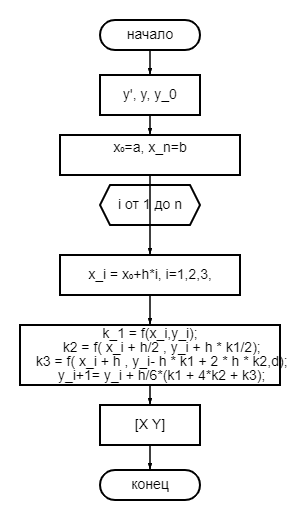
\includegraphics[scale=0.7]{diagram (6).png} 
\end{center}
\caption{Блок-схема метода Рунге-Кутты третьего порядка} \label{Рис1}
\end{figure}

\begin{figure}[h!]
\begin{center}
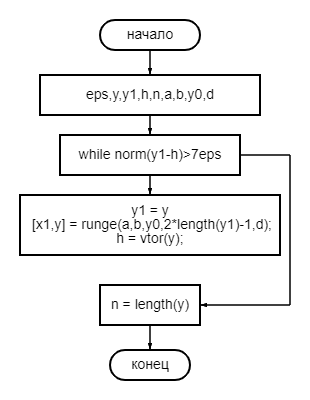
\includegraphics[scale=0.7]{diagram (6)1.png} 
\end{center}
\caption{Блок-схема правила Рунге} \label{Рис2}
\end{figure}
\newpage
\section{Численный анализ решения задачи}

\begin{figure}[h!]
\begin{center}
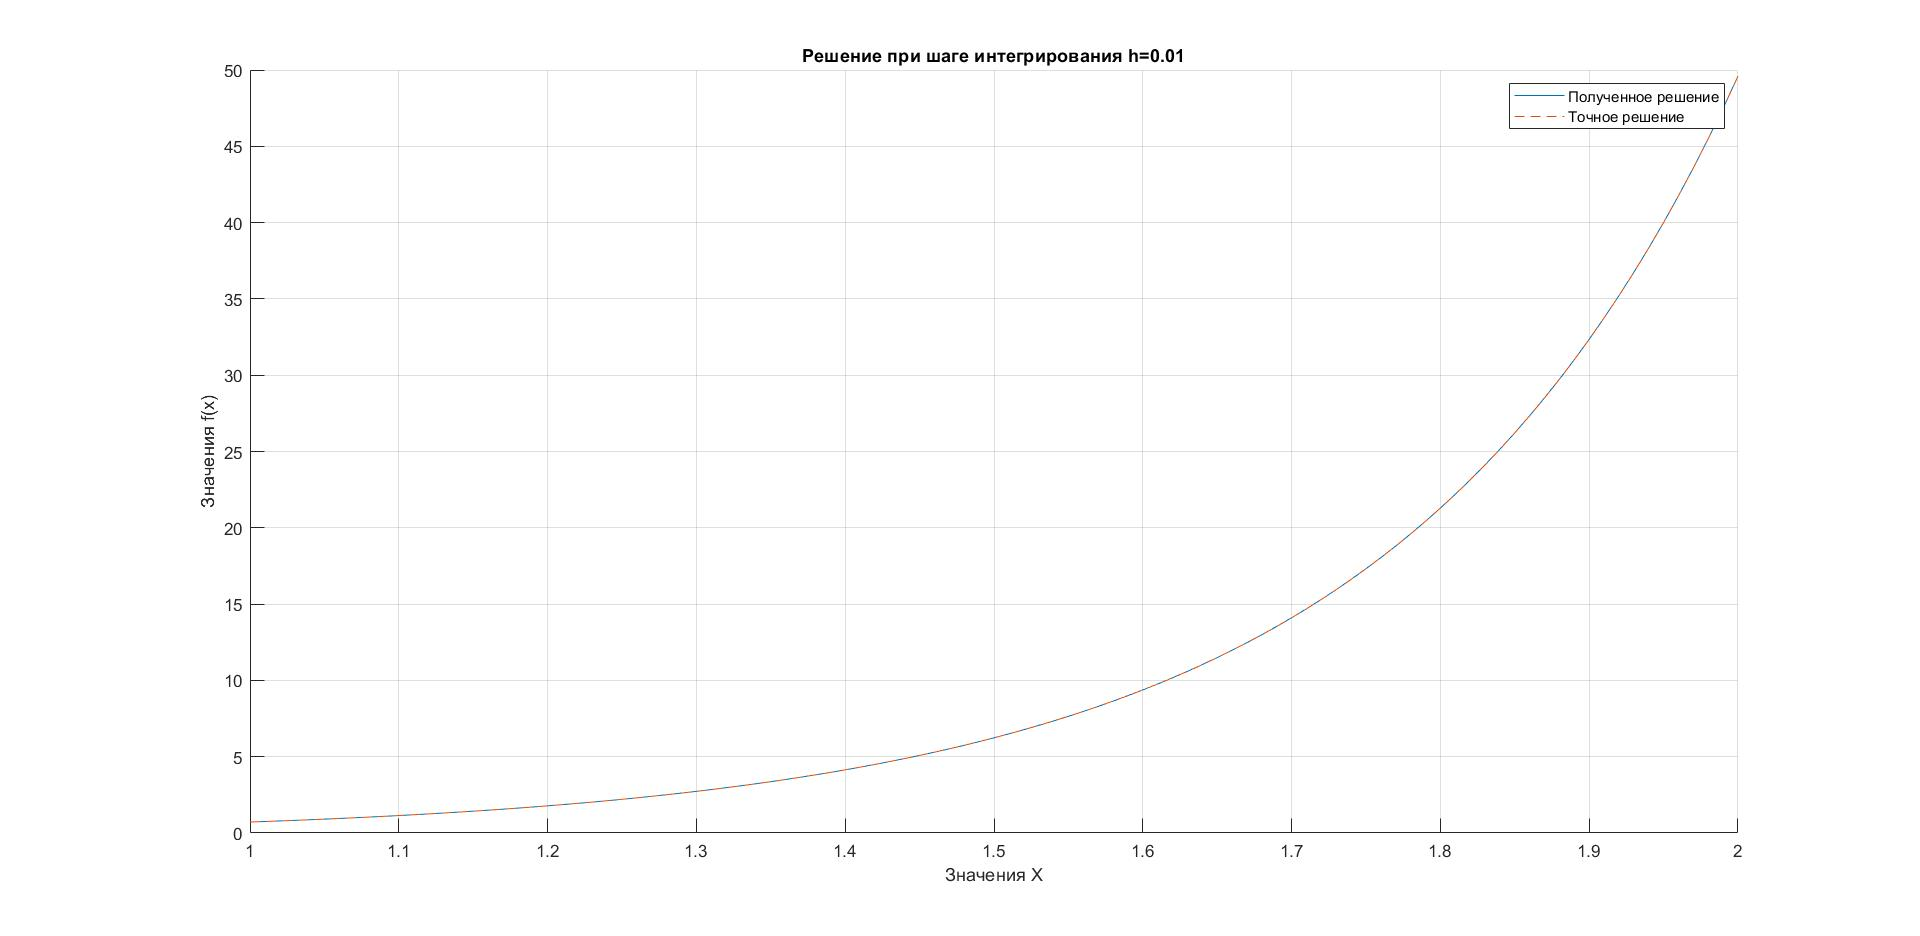
\includegraphics[scale=0.3]{решение при шаге интегрирования 0.01.jpg} 
\end{center}
\caption{Решение при шаге 0.01} \label{Рис3}
\end{figure}

\begin{figure}[h!]
\begin{center}
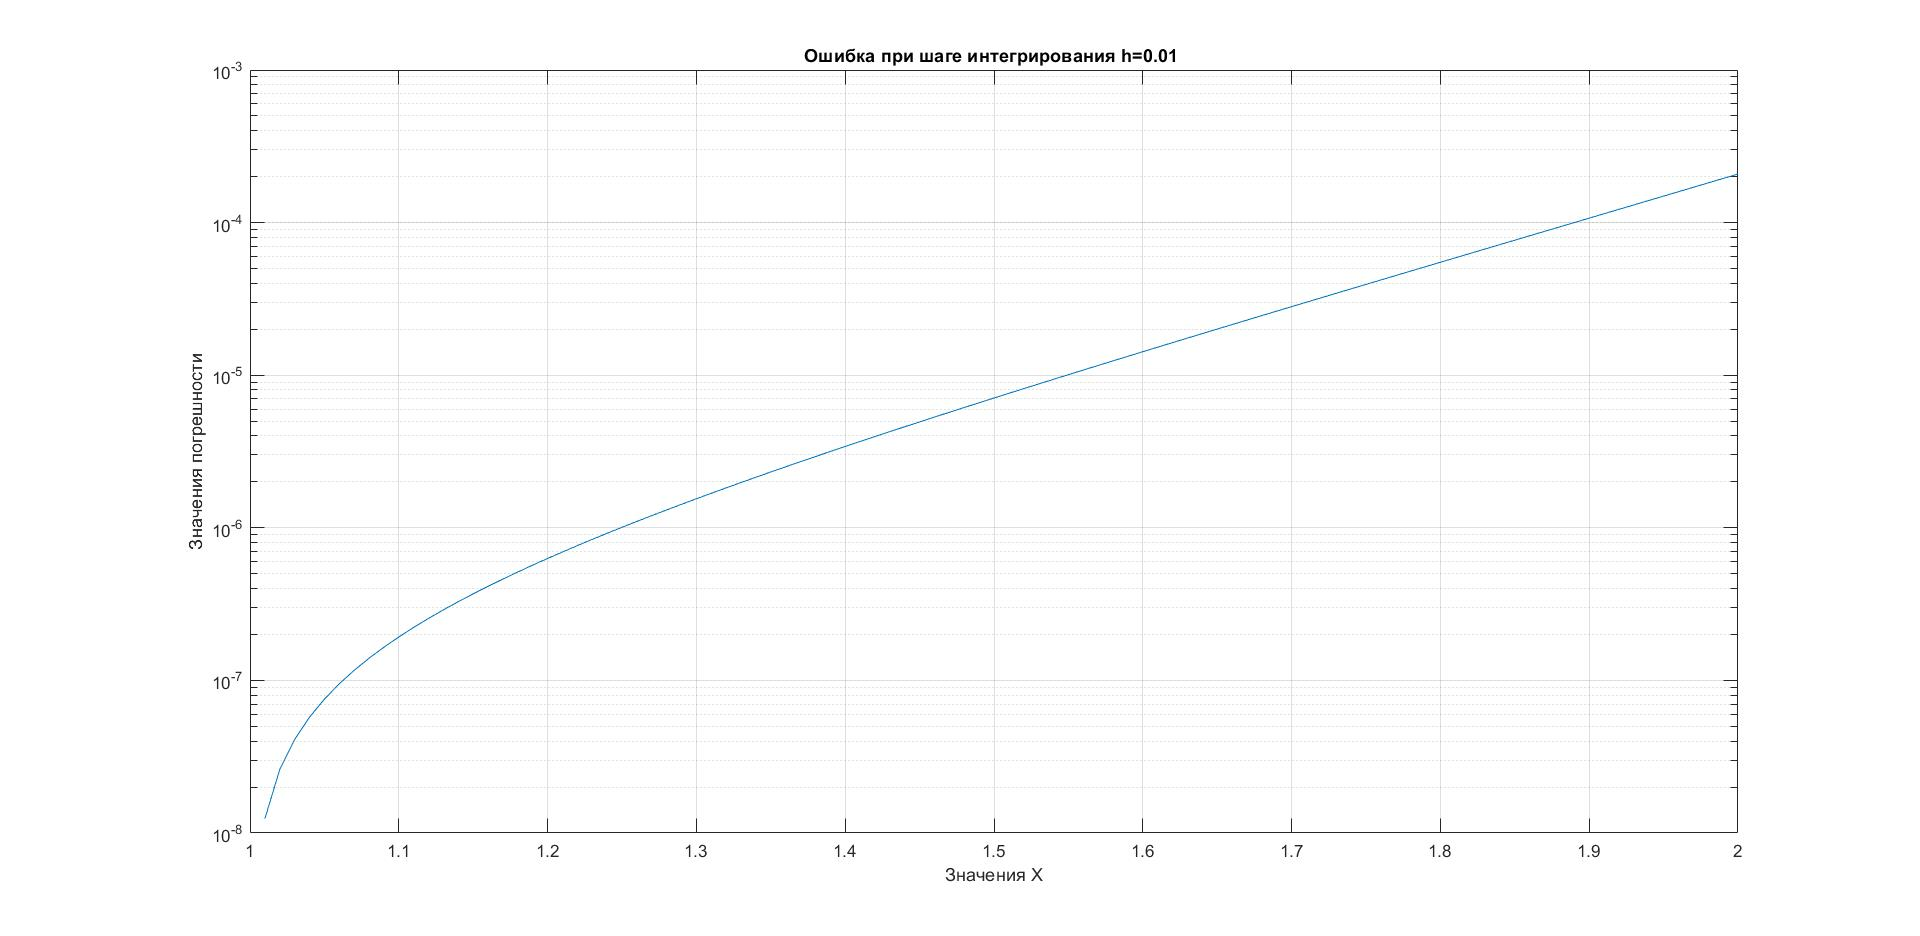
\includegraphics[scale=0.3]{ошибка при шаге интегрирования 0.01.jpg} 
\end{center}
\caption{Ошибка при шаге 0.01} \label{Рис4}
\end{figure}

Для начала хотелось бы представить график решения ОДУ при шаге 0.01. Как можно увидеть из рисунка \ref{Рис3} решение получается точным, но стоит всё же обратиться к отдельному графику погрешности для того же фиксированного шага. Для этого обратим внимание на график на рисунке \ref{Рис4} как видим, в начале отрезка меньшая погрешность, которая возрастает к его концу.



\subsection{Исследование зависимости погрешности от различных данных} 

\begin{figure}[h!]
\begin{center}
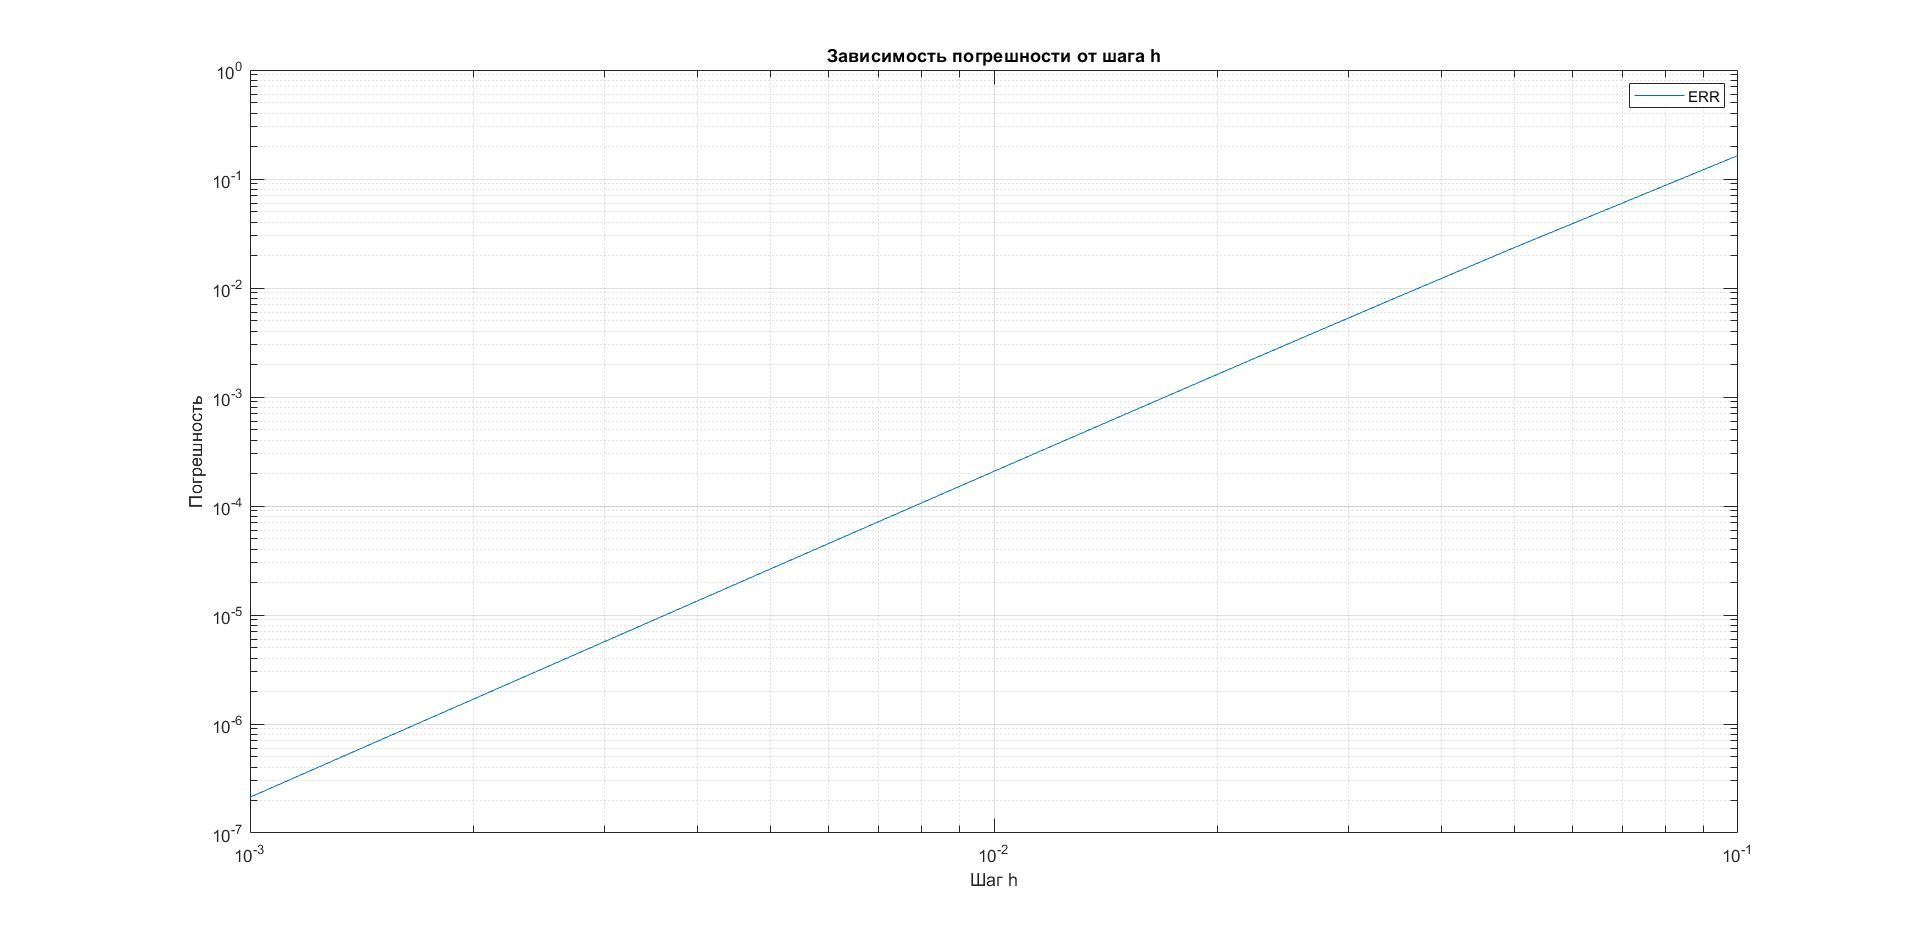
\includegraphics[scale=0.3]{зависимость погрешности от шага н.jpg} 
\end{center}
\caption{Зависимость погрешности от шага} \label{Рис5}
\end{figure}
Теперь обратимся к исследованию зависимости погрешности ошибки от шага. На рисунке $\ref{Рис5}$ изображен график по оси абсцисс которого отмечается шаг h, по оси ординат максимальная погрешнось при заданном шаге.Шаг меняется от 0.1 до 0.01, как несложно заметить,чем больше шаг, тем больше погрешность.


\begin{figure}[h!]
\begin{center}
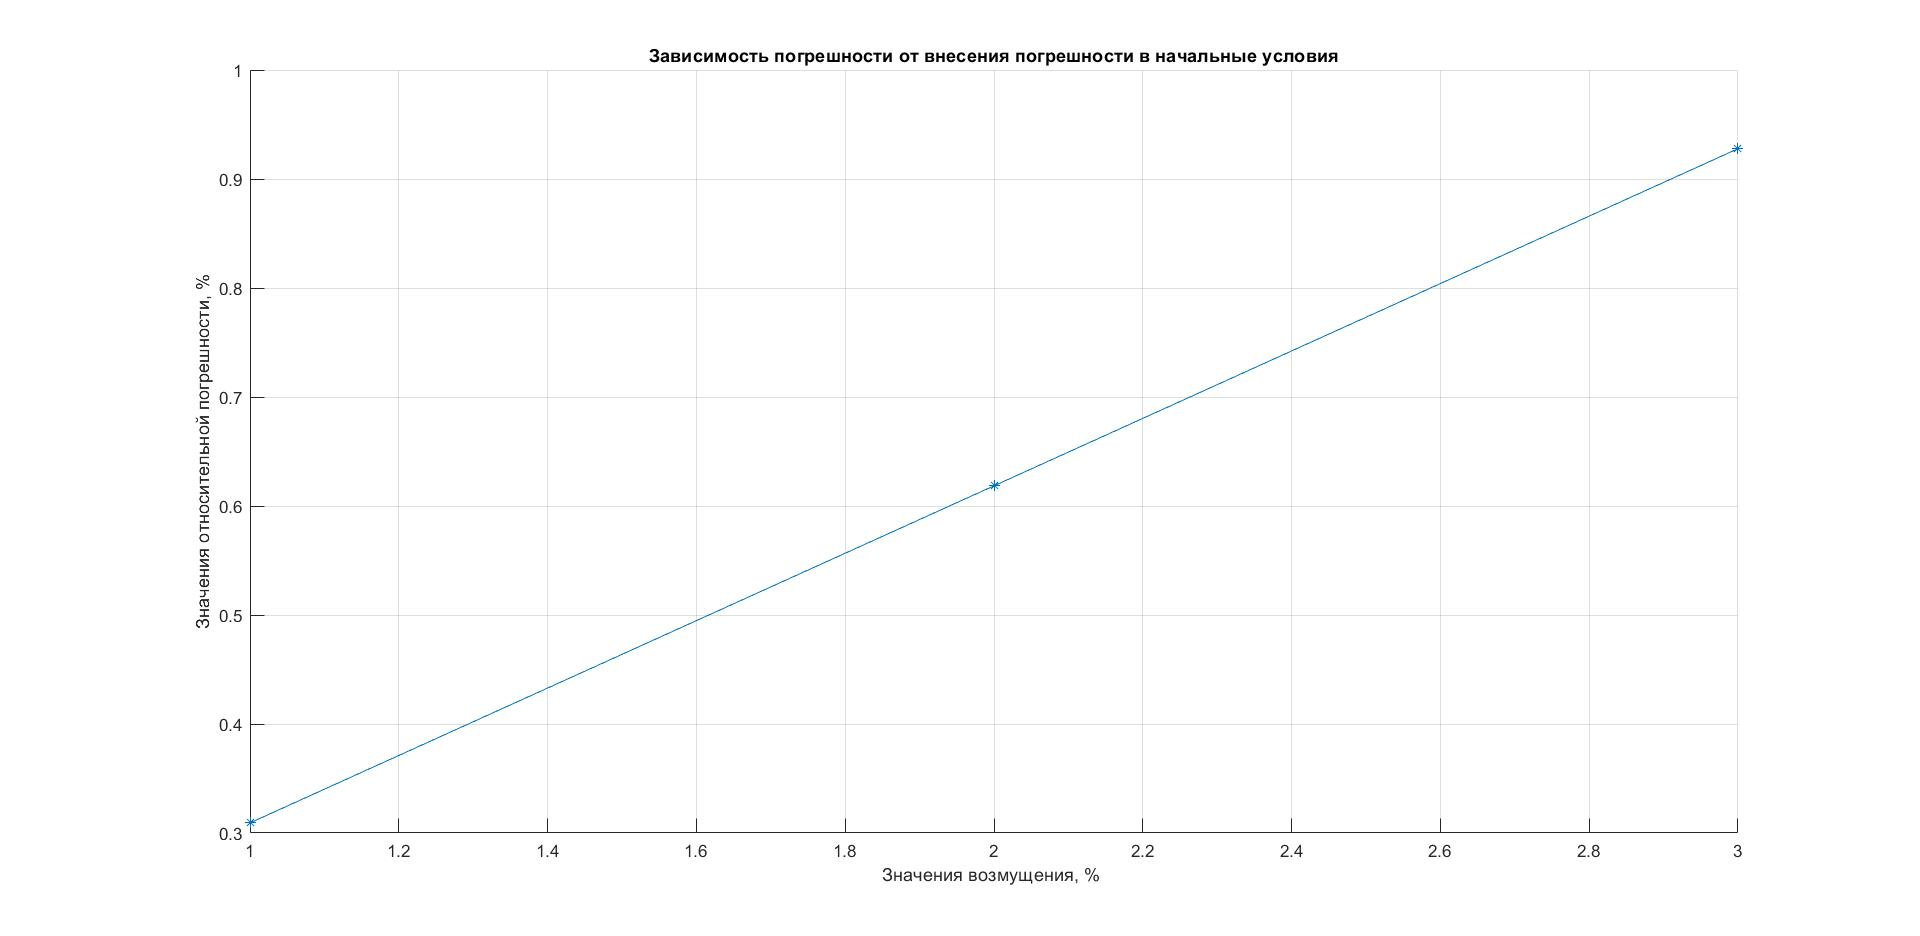
\includegraphics[scale=0.3]{зависимость погрешности от внесения возмущения в начальные условия.jpg}  
\end{center}
\caption{Зависимость погрешности от внесения возмущения в начальные условия} \label{Рис6}
\end{figure}

\begin{figure}[h!]
\begin{center}
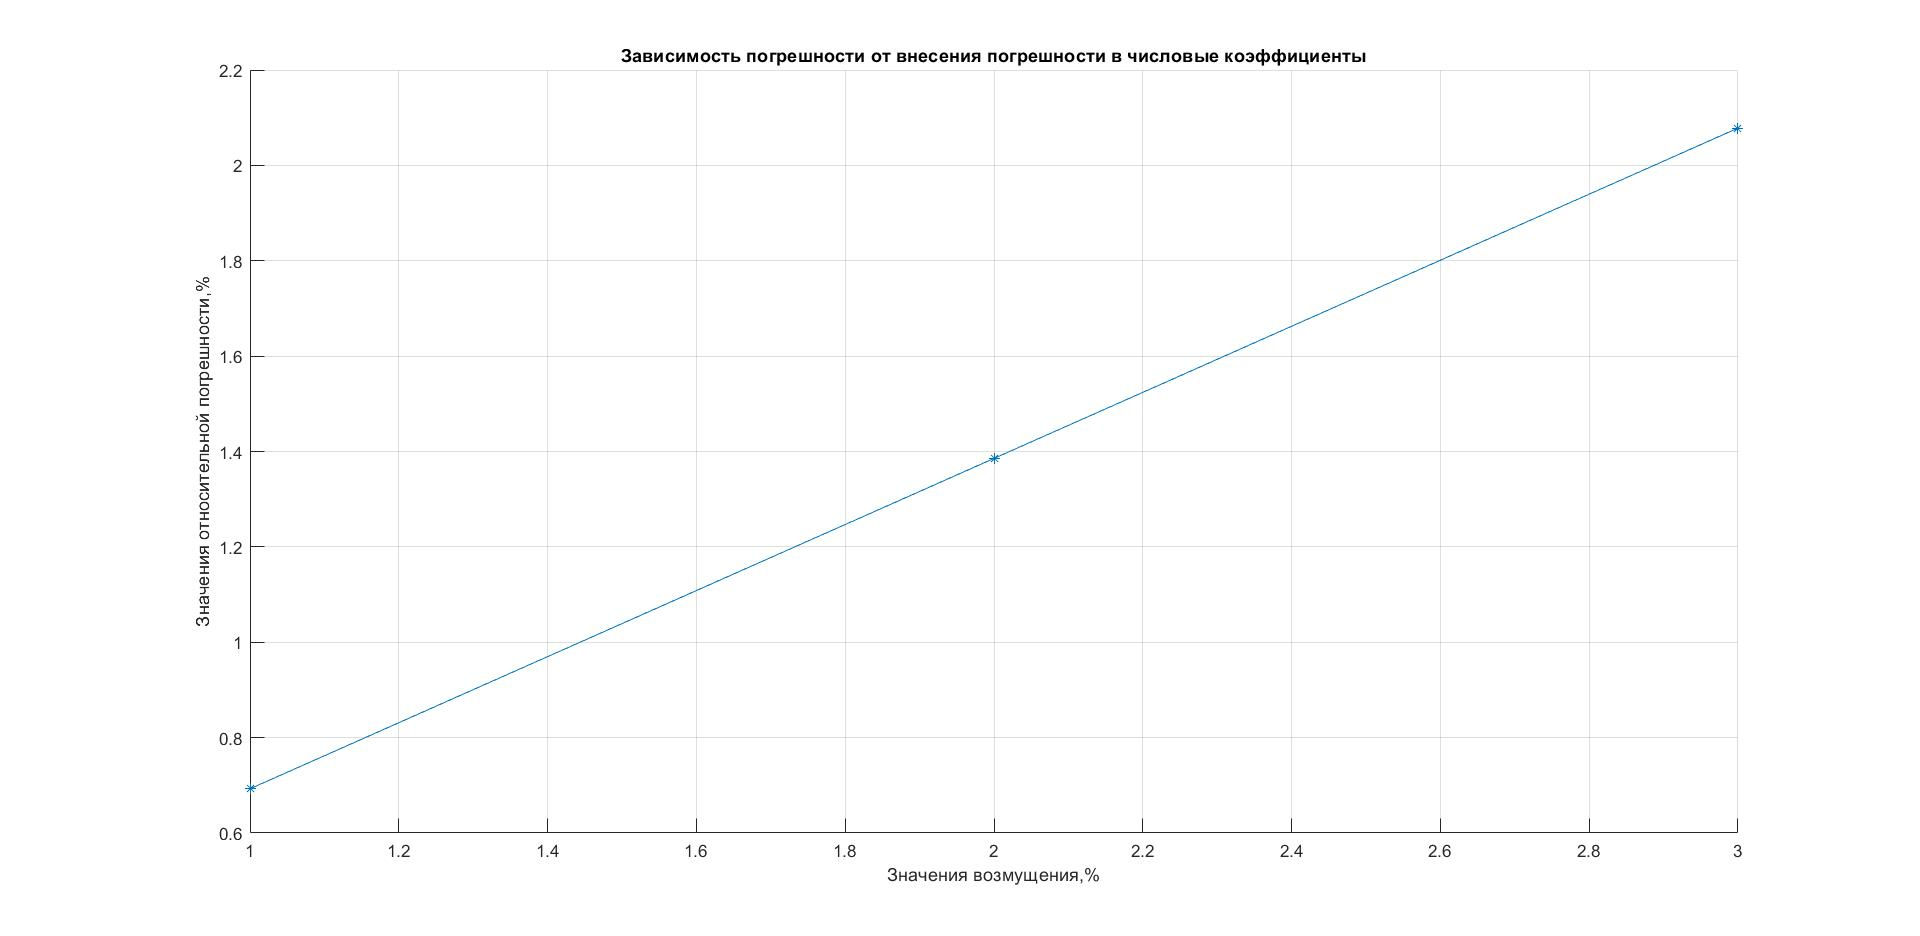
\includegraphics[scale=0.3]{зависимость погрешности от внесения возмущения в числовые коэффициенты.jpg}   
\end{center}
\caption{Зависимость погрешности от внесения возмущения в числовые коэффициенты} \label{Рис7}
\end{figure}
Далее рассмотрим, как ведет себя погрешность при возмущении некоторых данных. Для начала рассмотрим зависимость погрешности от внесения возмущения в начальные данные. Посмотрим на графики на рисунках $\ref{Рис6}$ и $\ref{Рис7}  $. По оси абсцисс будем отмечать возмущение в процентах, по оси ординат отметим относительную ошибку в процентах. На графике рисунка \ref{Рис5} изображена погрешность полученная при внесении возмущения в начальные условия, как можем заметить процент ошибки достаточно мал, на рисунке \ref{Рис7} отмечена относительная погрешность, полученная при внесении возмущения в числовые коэффициенты, здесь же процент ошибки мал, но все же чуть больше, чем при внесении возмущения в начальные данные.

\subsection{Сравнение теоретической и фактической точности} 

\begin{figure}[h!]
\begin{center}
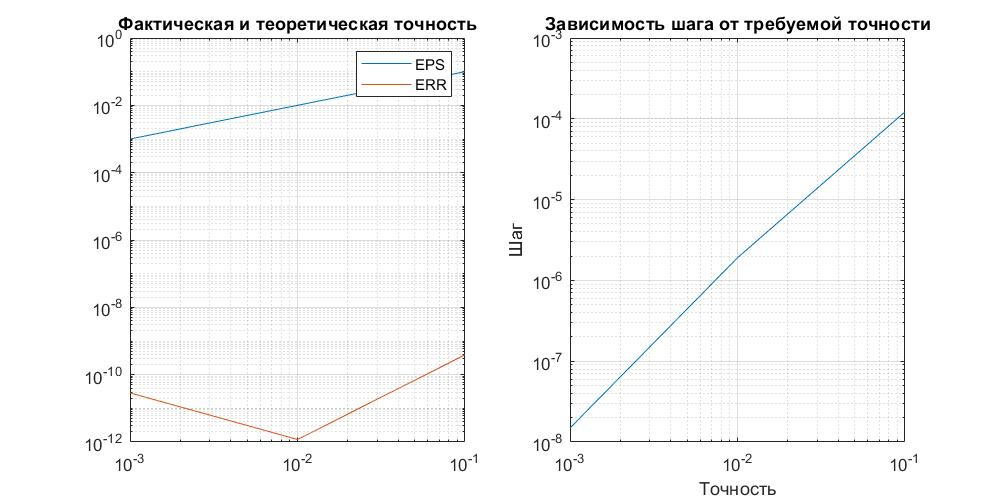
\includegraphics[scale=0.5]{правило рунге.jpg} 
\end{center}
\caption{Графики, полученные с использованием правила Рунге} \label{Рис8}
\end{figure}
На первом графике на рисунке $\ref{Рис8}$ можно отметить, что фактическая точность не превышает теоретической, что и ожидалось.Провести исследование получается только до требуемой точности равной $10^{-3}$. Далее проверить не позволяет программа, но даже при таком исследовании можно наблюдать, что точность достаточно хороша.  На втором графике того же рисунка мы видим, какой шаг необходимо использовать для получения нужной точности. Как можно заметить, чем меньший шаг мы берем, тем более "хорошее" значение точности мы получаем.\\


\newpage
\section{Краткие выводы} 

\begin{itemize}
  \item Метод Рунге-Кутты третьего порядка дает достаточно точные результаты, если взять достаточно маленький шаг.
  \item Все исследования удовлетворили предварительному анализу.
  \item Можно заметить, что метод является достаточно устойчивым, потому что вносимые возмущения не дали большую погрешность. 
  \end{itemize}


\end{document} % КОНЕЦ ДОКУМЕНТА !

